\section{eo\-Es\-Standard\-Xover$<$ EOT $>$ Class Template Reference}
\label{classeo_es_standard_xover}\index{eoEsStandardXover@{eoEsStandardXover}}
Standard (i.e.  


{\tt \#include $<$eo\-Es\-Standard\-Xover.h$>$}

Inheritance diagram for eo\-Es\-Standard\-Xover$<$ EOT $>$::\begin{figure}[H]
\begin{center}
\leavevmode
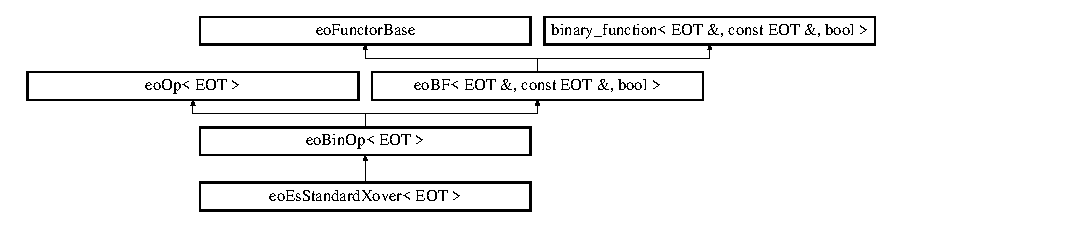
\includegraphics[height=2.60163cm]{classeo_es_standard_xover}
\end{center}
\end{figure}
\subsection*{Public Types}
\begin{CompactItemize}
\item 
typedef EOT::Fitness {\bf Fit\-T}\label{classeo_es_standard_xover_w0}

\end{CompactItemize}
\subsection*{Public Member Functions}
\begin{CompactItemize}
\item 
{\bf eo\-Es\-Standard\-Xover} ({\bf eo\-Bin\-Op}$<$ double $>$ \&\_\-cross\-Obj, {\bf eo\-Bin\-Op}$<$ double $>$ \&\_\-cross\-Mut)\label{classeo_es_standard_xover_a0}

\begin{CompactList}\small\item\em (Default) Constructor. \item\end{CompactList}\item 
virtual std::string {\bf class\-Name} () const \label{classeo_es_standard_xover_a1}

\begin{CompactList}\small\item\em The class name. Used to display statistics. \item\end{CompactList}\item 
bool {\bf operator()} ({\bf EOT} \&\_\-eo1, const {\bf EOT} \&\_\-eo2)\label{classeo_es_standard_xover_a2}

\begin{CompactList}\small\item\em modifies one parents in the populator using a second parent \item\end{CompactList}\end{CompactItemize}
\subsection*{Private Member Functions}
\begin{CompactItemize}
\item 
bool {\bf cross\_\-self\_\-adapt} ({\bf eo\-Es\-Simple}$<$ Fit\-T $>$ \&\_\-parent1, const {\bf eo\-Es\-Simple}$<$ Fit\-T $>$ \&\_\-parent2)\label{classeo_es_standard_xover_d0}

\item 
bool {\bf cross\_\-self\_\-adapt} ({\bf eo\-Es\-Stdev}$<$ Fit\-T $>$ \&\_\-parent1, const {\bf eo\-Es\-Stdev}$<$ Fit\-T $>$ \&\_\-parent2)\label{classeo_es_standard_xover_d1}

\item 
bool {\bf cross\_\-self\_\-adapt} ({\bf eo\-Es\-Full}$<$ Fit\-T $>$ \&\_\-parent1, const {\bf eo\-Es\-Full}$<$ Fit\-T $>$ \&\_\-parent2)\label{classeo_es_standard_xover_d2}

\end{CompactItemize}
\subsection*{Private Attributes}
\begin{CompactItemize}
\item 
{\bf eo\-Random\-Select}$<$ {\bf EOT} $>$ {\bf sel}\label{classeo_es_standard_xover_r0}

\item 
{\bf eo\-Bin\-Op}$<$ double $>$ \& {\bf cross\-Obj}\label{classeo_es_standard_xover_r1}

\item 
{\bf eo\-Bin\-Op}$<$ double $>$ \& {\bf cross\-Mut}\label{classeo_es_standard_xover_r2}

\end{CompactItemize}


\subsection{Detailed Description}
\subsubsection*{template$<$class EOT$>$ class eo\-Es\-Standard\-Xover$<$ EOT $>$}

Standard (i.e. 

{\bf eo\-Bin\-Op}{\rm (p.\,\pageref{classeo_bin_op})}) crossover operator for ES genotypes. Uses some Atom crossovers to handle both the object variables and the mutation strategy parameters It is an {\bf eo\-Bin\-Op}{\rm (p.\,\pageref{classeo_bin_op})} and has to be wrapped into an {\bf eo\-Gen\-Op}{\rm (p.\,\pageref{classeo_gen_op})} before being used like the global version 



Definition at line 46 of file eo\-Es\-Standard\-Xover.h.

The documentation for this class was generated from the following file:\begin{CompactItemize}
\item 
eo\-Es\-Standard\-Xover.h\end{CompactItemize}
